\documentclass[12pt,table,t]{beamer}

% Packages
\usepackage{xcolor}
\usepackage{eulervm}
\usepackage[utf8]{inputenc}


% Theme
\mode<presentation>
{
  \usetheme{Honefoss}
%  \setbeamercovered{transparent}
  \setbeamertemplate{blocks}[rounded]
  \AtBeginPart{\frame[c]{\partpage}}
}

\logooff
\newcommand{\comment}[1]{{\slshape\color{kvred}#1}}

\title{Lytt til Kvasarer og\\Skyt Satellitter med Laser}
\author{Geir Arne Hjelle}
\date{FOSS4G Norge, 18.\ Oktober 2018}
\titlegraphic{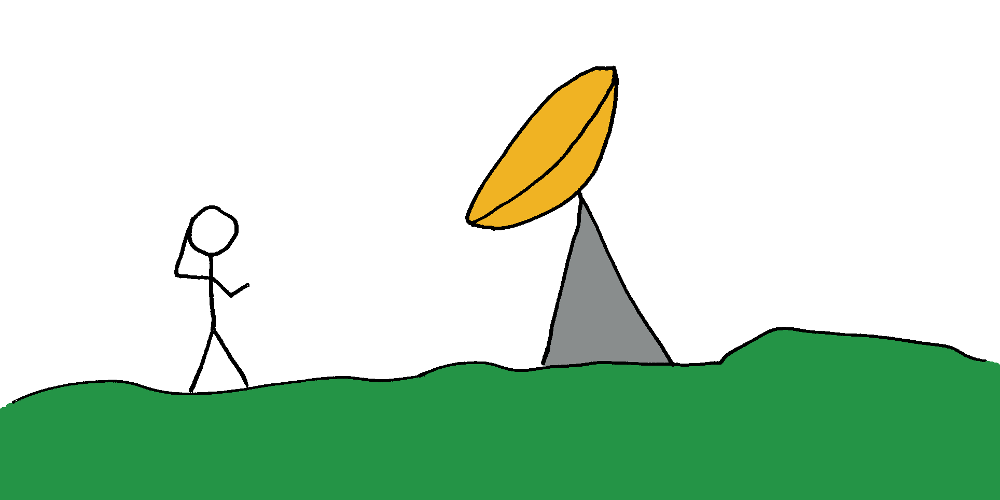
\includegraphics[width=\paperwidth]{figure/vlbi}}

\begin{document}
\frame[plain]{\titlepage}

\part{Hvorfor?}

\begin{frame}[c]{Problemet}
  \begin{center}
    \includegraphics<1>[width=\textwidth]{figure/altimetry_01}
    \includegraphics<2>[width=\textwidth]{figure/altimetry_02}
    \includegraphics<3>[width=\textwidth]{figure/altimetry_03}
    \includegraphics<4>[width=\textwidth]{figure/altimetry_04}
    \includegraphics<5>[width=\textwidth]{figure/altimetry_05}
    \includegraphics<6>[width=\textwidth]{figure/gps_01}
    \includegraphics<7>[width=\textwidth]{figure/gps_02}
    \includegraphics<8>[width=\textwidth]{figure/gps_03}
  \end{center}
\end{frame}


\begin{frame}[c]{Løsningen}
  \begin{center}
    \includegraphics<1>[width=\textwidth]{figure/reference_system}
  \end{center}

  Et \textbf{referansesystem}\footnote{Essensielt et koordinatsystem basert på referansepunkter}
\end{frame}


\begin{frame}[c]{Løsningen}
  \begin{center}
    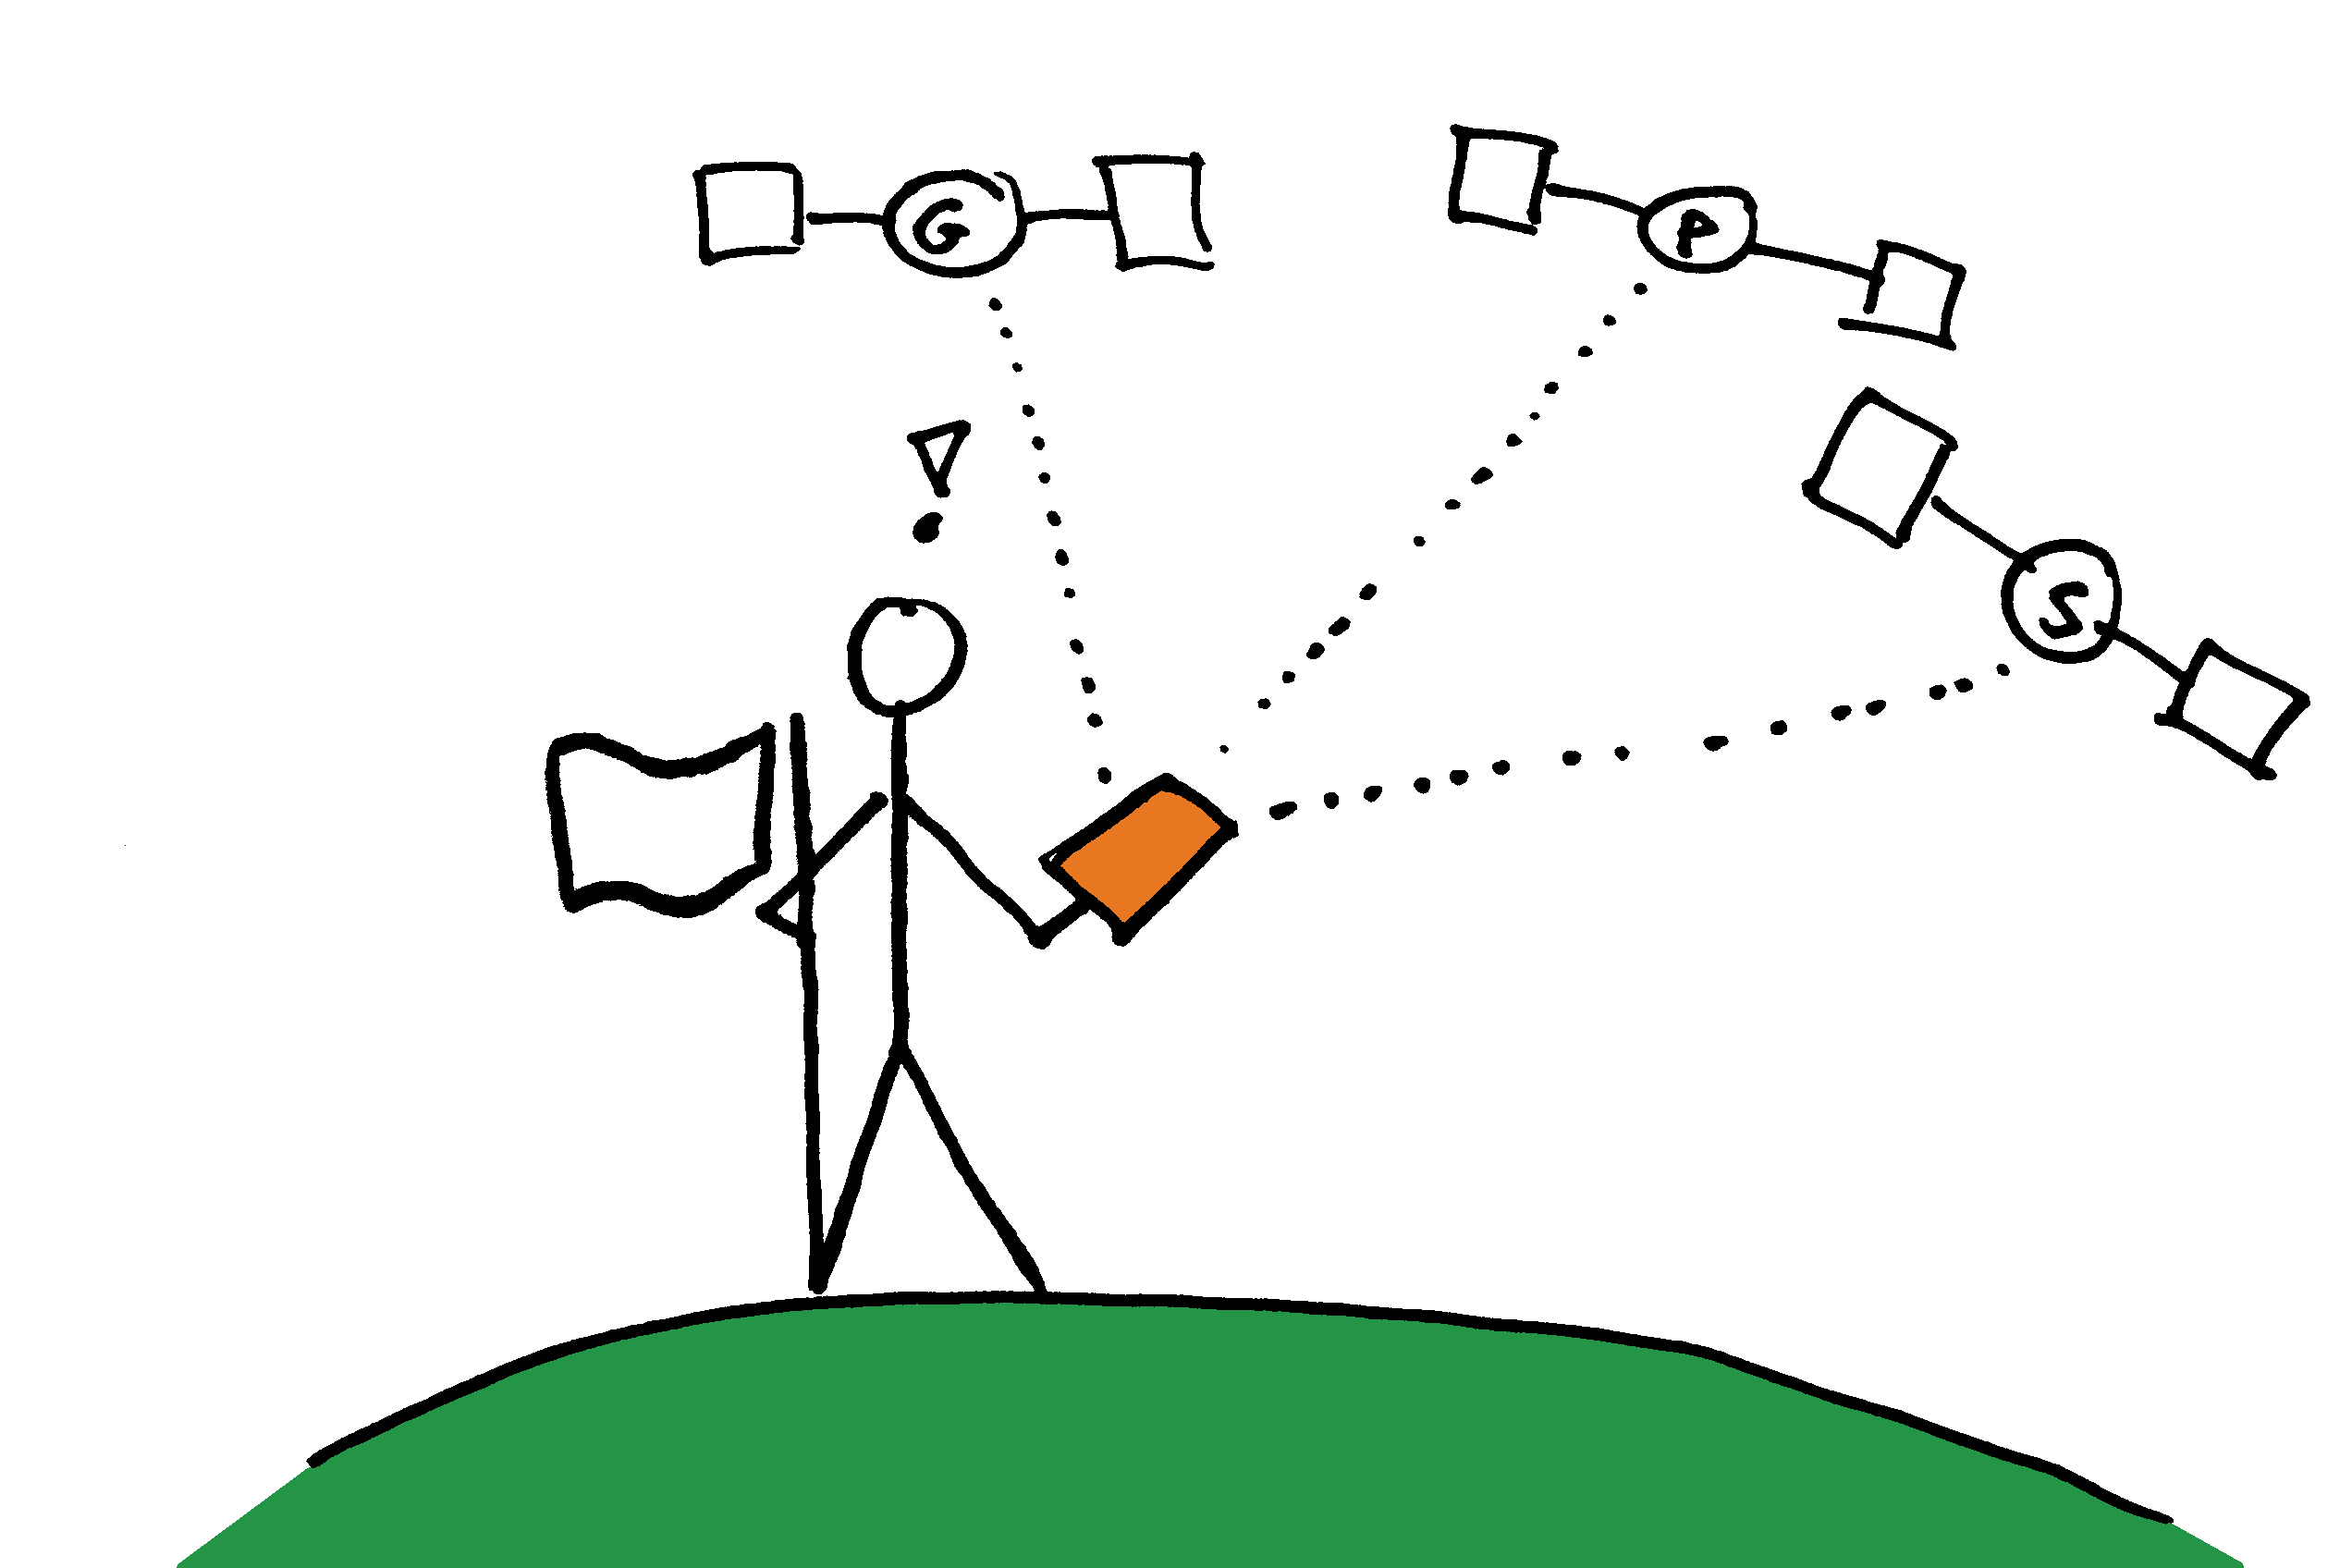
\includegraphics[width=\textwidth]{figure/gps_04}
  \end{center}
\end{frame}


\begin{frame}[c]{Løsningen}
  Men det er ikke trivielt å realisere et slikt referansesystem ... 

  \vspace*{4ex}
  \begin{center}
    \includegraphics<1>[width=\textwidth]{figure/origin}
  \end{center}
\end{frame}


\begin{frame}[c]{Løsningen}
  Ønsker en \textbf{referanseramme} som er:

  \begin{itemize}
  \item<2-> presis
  \item<3-> stabil over tid
  \end{itemize}

  \begin{center}
    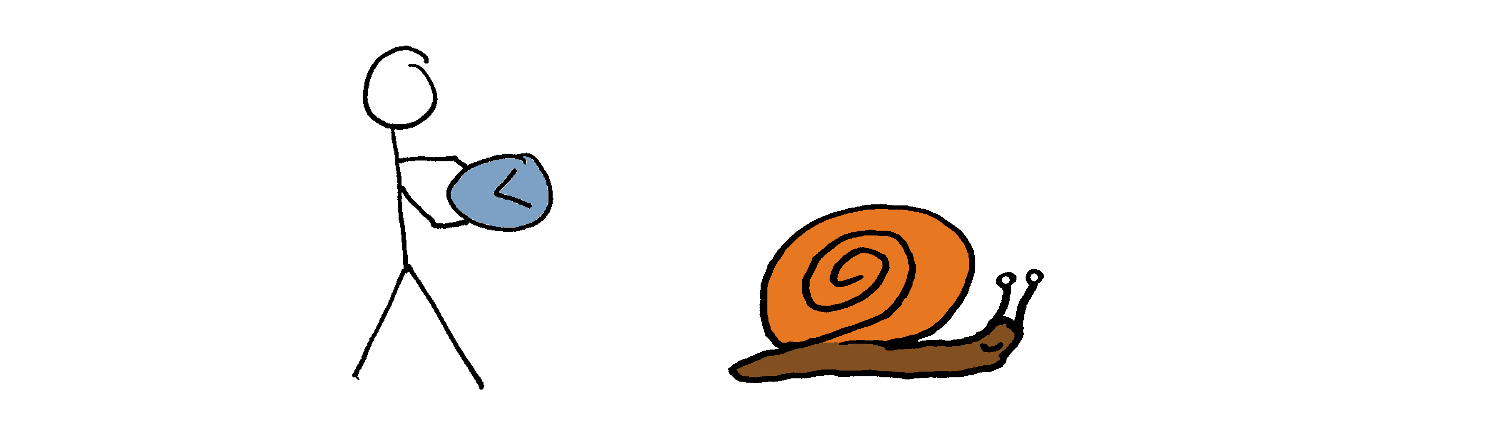
\includegraphics[width=\textwidth]{figure/time}
  \end{center}
\end{frame}


\begin{frame}[c]{Utfordringer}

  \begin{itemize}
  \item<2-> Tektoniske plater flytter seg
  \item<3-> Landheving og stigende havnivå
  \item<4-> Jordskjelv
  \end{itemize}
  
  \begin{center}
    \includegraphics<-1>[width=.3\textwidth]{figure/earth_sq}
    \includegraphics<2->[width=.3\textwidth]{figure/plate_drift_sq}
    \includegraphics<-2>[width=.3\textwidth]{figure/earth_sq}
    \includegraphics<3->[width=.3\textwidth]{figure/uplift}
    \includegraphics<-3>[width=.3\textwidth]{figure/earth_sq}
    \includegraphics<4->[width=.3\textwidth]{figure/earthquake_sq}
  \end{center}
\end{frame}


\begin{frame}{Løsninger}

  \begin{itemize}
  \item Lokale systemer
  \end{itemize}
  
  \begin{center}
    \includegraphics<1>[width=\textwidth]{figure/local_system_01}
    \includegraphics<2>[width=\textwidth]{figure/local_system_02}
  \end{center}
\end{frame}


\begin{frame}{Løsninger}

  \begin{itemize}
  \item Koordinater som flytter på seg
  \end{itemize}
  
  \begin{center}
    \includegraphics<1>[width=\textwidth]{figure/snail_01}
    \includegraphics<2>[width=\textwidth]{figure/snail_02}
    \includegraphics<3>[width=\textwidth]{figure/snail_03}
    \includegraphics<4>[width=\textwidth]{figure/snail_04}
    \includegraphics<5>[width=\textwidth]{figure/snail_05}
  \end{center}
\end{frame}

\part{Hva?}

\begin{frame}[c]{ITRF}

  \begin{itemize}
  \item Den Internasjonale Terrestriske Referanserammen (ITRF)
  \end{itemize}
    
  \begin{center}
    \includegraphics<1>[width=\textwidth]{figure/itrf_01}
    \includegraphics<2>[width=\textwidth]{figure/itrf_02}
    \includegraphics<3>[width=\textwidth]{figure/itrf_03}
  \end{center}
\end{frame}

\part{Hvordan?}

\begin{frame}[c]{Internasjonalt Samarbeid}
  \begin{center}
    \includegraphics<1>[width=\textwidth]{figure/cooperation_01}
    \includegraphics<2>[width=\textwidth]{figure/cooperation_02}
    \includegraphics<3>[width=\textwidth]{figure/cooperation_03}
    \includegraphics<4>[width=\textwidth]{figure/cooperation_04}
    \includegraphics<5>[width=\textwidth]{figure/cooperation_05}
  \end{center}

  \begin{itemize}
  \item ITRF lages basert på observasjoner fra fire forskjellige romgeodetiske teknikker
    \begin{itemize}
    \item<2-> VLBI -- Very Long Baseline Interferometry
    \item<3-> SLR -- Satellite Laser Ranging
    \item<4-> GNSS -- Global Navigation Satellite Systems (e.g. GPS)
    \item<5-> DORIS -- Doppler Orbitography and Radiopositioning
    \end{itemize}
  \end{itemize}
\end{frame}


\begin{frame}[c]{Stadig Flere Utfordringer}

  \begin{itemize}
  \item Jorda roterer
  \end{itemize}
  
  \begin{center}
    \includegraphics<1>[width=0.3\textwidth]{figure/earth_rotates_01}
    \includegraphics<2>[width=0.3\textwidth]{figure/earth_rotates_02}
    \includegraphics<3>[width=0.3\textwidth]{figure/earth_rotates_03}
    \includegraphics<4>[width=0.3\textwidth]{figure/earth_rotates_04}
    \includegraphics<5>[width=0.3\textwidth]{figure/earth_rotates_05}
    \includegraphics<6>[width=0.3\textwidth]{figure/earth_rotates_06}
    \includegraphics<7>[width=0.3\textwidth]{figure/earth_rotates_07}
    \includegraphics<8>[width=0.3\textwidth]{figure/earth_rotates_08}
    \includegraphics<9>[width=0.3\textwidth]{figure/earth_rotates_01}
  \end{center}

  \begin{itemize}
  \item<9-> Fest referansesystemet til jorda med $z$ som rotasjonsakse
  \end{itemize}
\end{frame}


\begin{frame}[c]{Stadig Flere Utfordringer}

  \begin{itemize}
  \item Jorda vingler
  \end{itemize}
  
  \begin{center}
    \includegraphics<1>[width=0.4\textwidth]{figure/cheers_01}
    \includegraphics<2>[width=0.3\textwidth]{figure/drunk_01}
    \includegraphics<3>[width=0.3\textwidth]{figure/drunk_02}
    \includegraphics<4>[width=0.3\textwidth]{figure/drunk_01}
    \includegraphics<5>[width=0.3\textwidth]{figure/drunk_02}
  \end{center}

  \begin{itemize}
  \item<5-> Gjør kontinuerlige oppdateringer av jordorienteringsparametre (EOP)
  \end{itemize}
\end{frame}


\begin{frame}[c]{VLBI}
  \begin{center}
    \includegraphics<1>[width=\textwidth]{figure/vlbi_concept_01}
    \includegraphics<2>[width=\textwidth]{figure/vlbi_concept_02}
    \includegraphics<3->[width=\textwidth]{figure/vlbi_concept_03}
  \end{center}

  \uncover<4->{
  Regn ut en \textbf{modell} hvor:
  \begin{itemize}
  \item stasjonsposisjoner antas kjente (ITRF)
  \item et a priori estimat av vinglingen er inkludert
  \end{itemize}}
\end{frame}


\begin{frame}[c]{VLBI}
  Residualet

  \begin{center}
    \textbf{obs} - \textbf{modell}
  \end{center}

  kan brukes for å estimere den faktiske vinglingen.

  \uncover<2>{
    \begin{center}
      
\includegraphics[width=.4\textwidth]{figure/cheers_02}
    \end{center}
  }
\end{frame}


\begin{frame}[c]{SLR}
  \begin{center}
    \includegraphics<1>[width=\textwidth]{figure/slr_concept_01}
    \includegraphics<2>[width=\textwidth]{figure/slr_concept_02}
    \includegraphics<3>[width=\textwidth]{figure/slr_concept_03}
  \end{center}
\end{frame}


\begin{frame}[c]{SLR}
  To anvendelser:

  \begin{center}
    \includegraphics<1>[width=\textwidth]{figure/lageos_01}
    \includegraphics<2>[width=\textwidth]{figure/lageos_02}
  \end{center}

  \uncover<2>{
    \begin{itemize}
    \item Stabile satellittbaner\\
      $\Rightarrow$ Kan beregne stasjonsposisjonen (ITRF)
  \end{itemize}}
\end{frame}


\begin{frame}[c]{SLR}
  To anvendelser:

    \begin{center}
    \includegraphics<1>[width=0.7\textwidth]{figure/altimetry_06}
  \end{center}

  \begin{itemize}
  \item Kjent stasjonsposisjon\\
    $\Rightarrow$ Kan beregne satellittbaner (remote sensing)
  \end{itemize}
\end{frame}


\part{Python}


\begin{frame}[c]{Where?}
  \begin{center}
    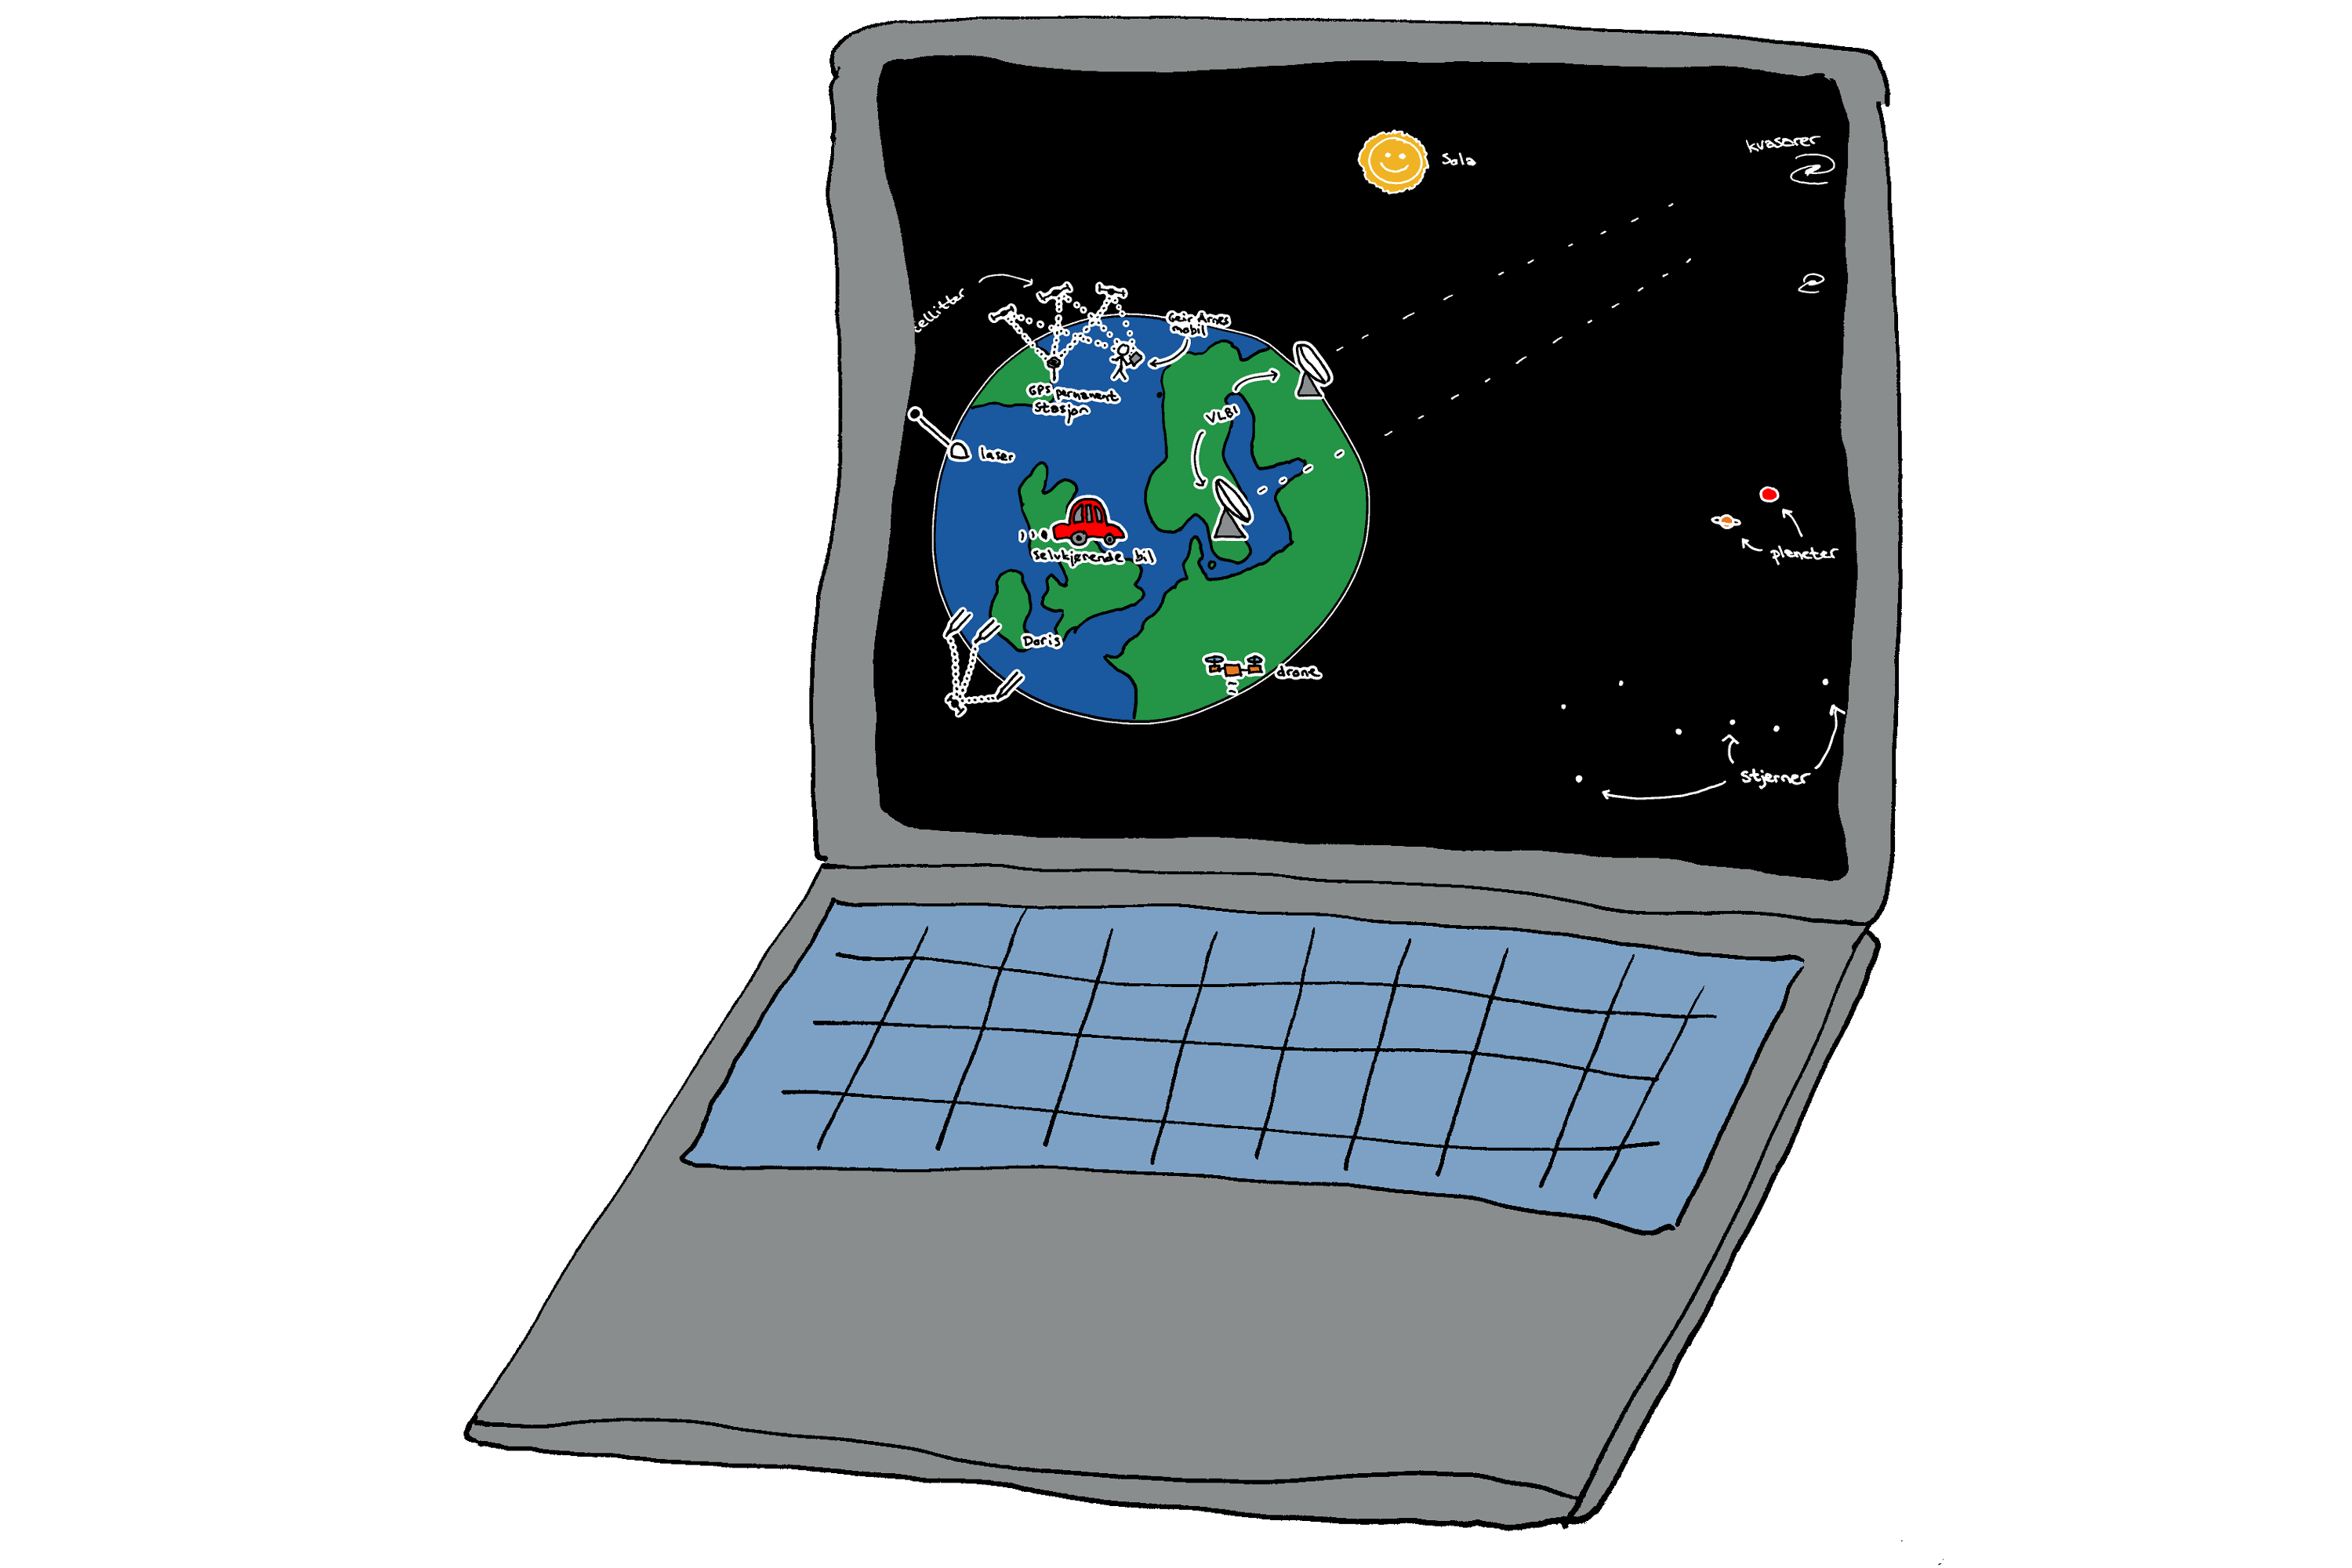
\includegraphics[width=\textwidth]{figure/where}
  \end{center}
\end{frame}


\begin{frame}[c]{Where?}
  \textbf{Where} er programvare som kan analysere VLBI-, SLR- og GNSS-data, og bidra til ITRF

  \begin{itemize}
  \item<2-> Python
  \item<3-> Open Source (\url{kartverket.github.io/where/})
  \item<4-> Er kanskje mest for spesielt interesserte
  \end{itemize}
\end{frame}


\begin{frame}[c]{There!}
  \begin{center}
    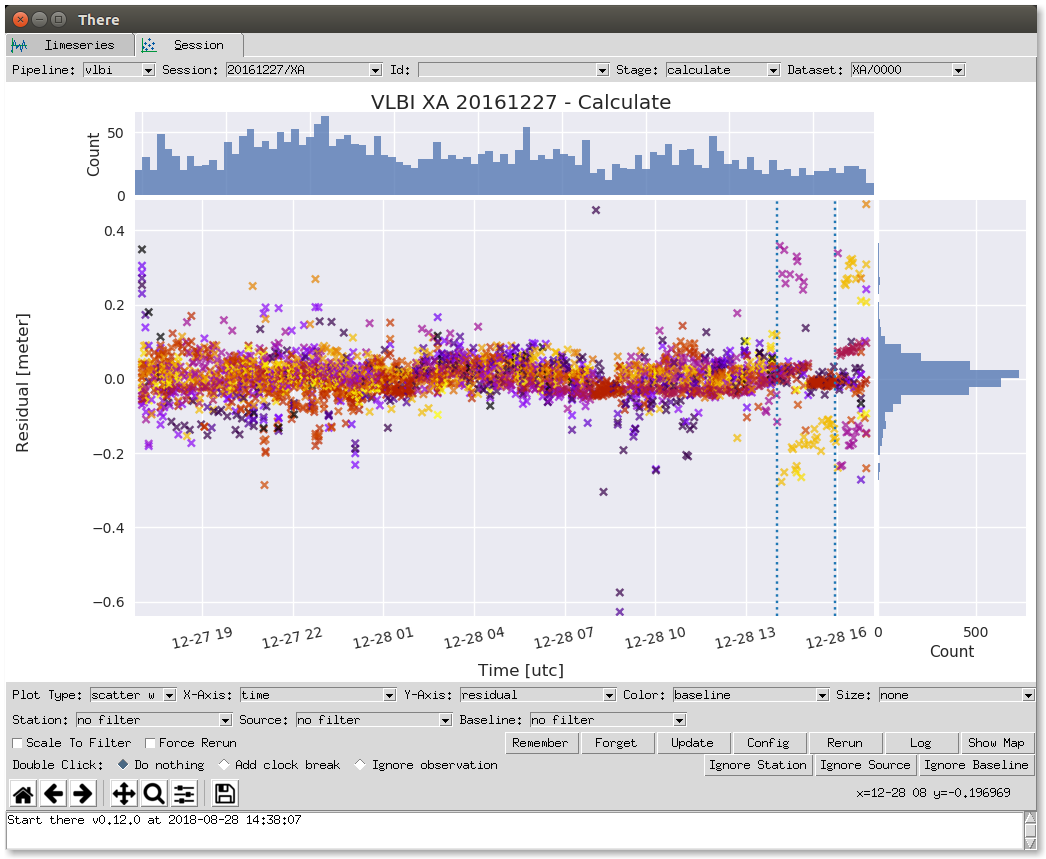
\includegraphics[width=0.4\textwidth]{figure/there_01} \hfil
    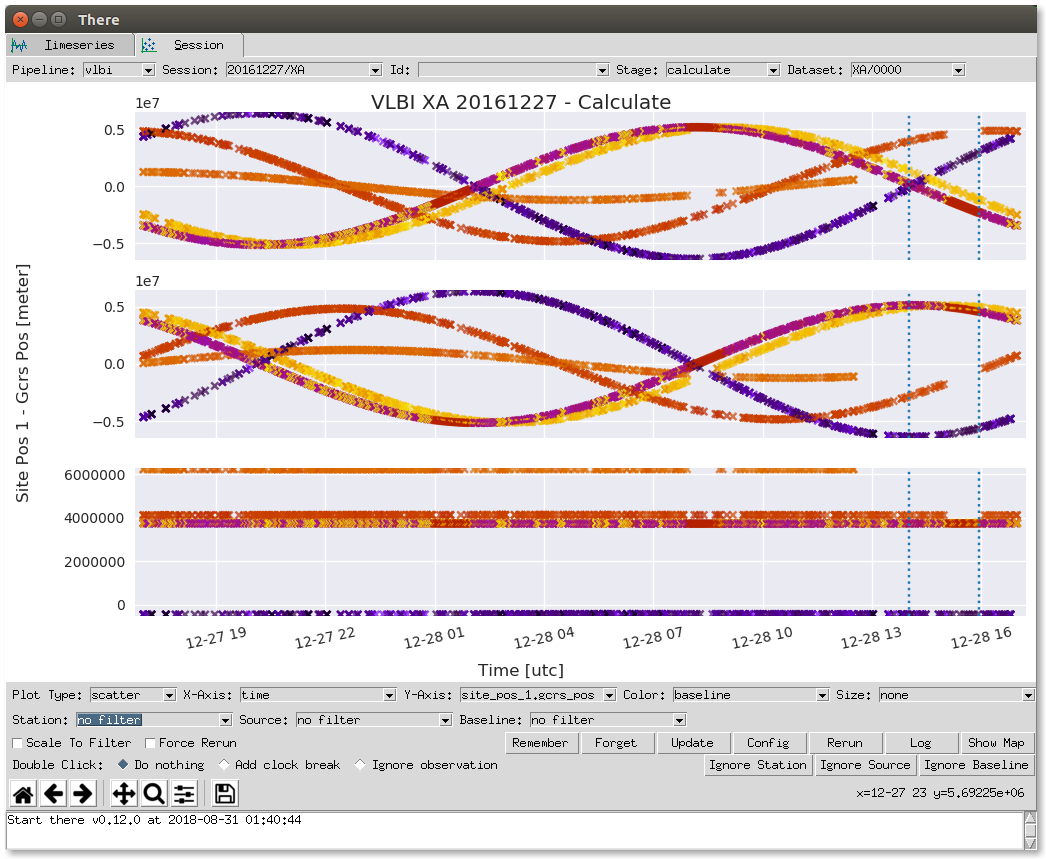
\includegraphics[width=0.4\textwidth]{figure/there_02}
  \end{center}

  Erfaringer:
  \begin{itemize}
  \item<2-> En stor takk til alle som bidrar til Open Source programvare!
  \item<3-> Ytelse: God pythonkode er raskere enn ikke-optimal fortrankode :)
  \item<4-> Visualisering er viktig, det finnes mange muligheter der ute
  \end{itemize}
\end{frame}


\begin{frame}[c]{Midgard}
  %% \begin{center}
  %%   \includegraphics<1>[width=\textwidth]{figure/midgard}
  %% \end{center}

  Gjenbrukbare komponenter i Where blir separert ut i et eget bibliotek: \textbf{Midgard}

  \begin{itemize}
  \item \texttt{pip install midgard}
  \item Datastrukturer for koordinater som flytter seg over tid
  \item Lesere for geodetiske filformater
  \end{itemize}
\end{frame}


\begin{frame}[c]{Takk for Oppmerksomheten}
  \begin{center}
    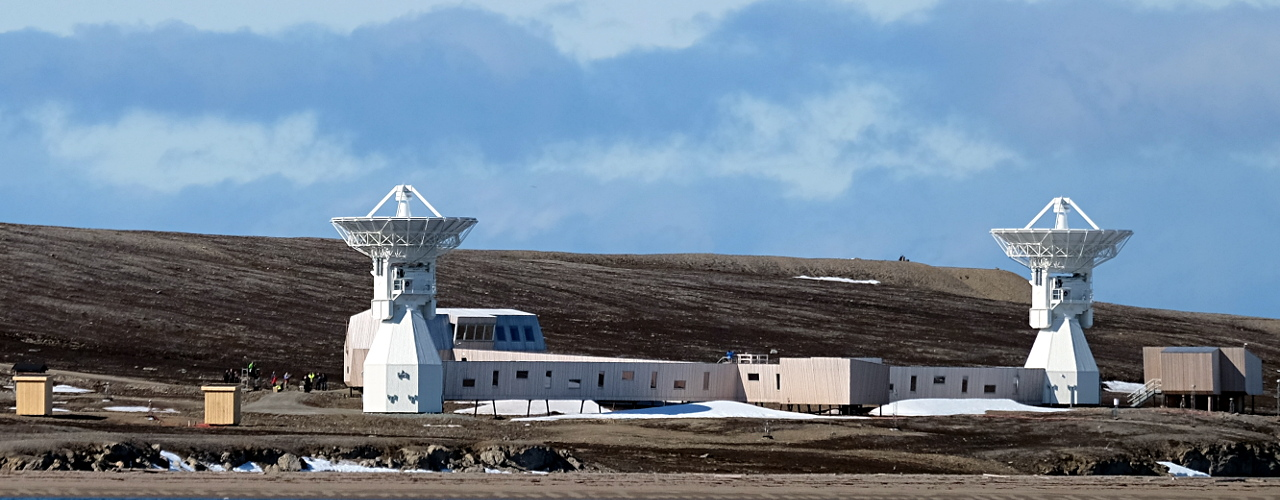
\includegraphics[width=\textwidth]{figure/ny_alesund}

    {\large\url{kartverket.github.io/where/}}
    \vspace*{1.3cm}

    
\includegraphics[height=1cm]{figure/logo_astropy} \hfil
    
\includegraphics[height=1cm]{figure/logo_numpy} \hfil
    
\includegraphics[height=1cm]{figure/logo_scipy} \hfil
    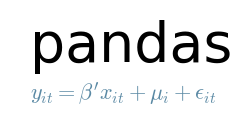
\includegraphics[height=1cm]{figure/logo_pandas} \hfil
    
\includegraphics[height=1cm]{figure/logo_cython} \hfil
    
\includegraphics[height=1cm]{figure/logo_f2py}
  \end{center}
\end{frame}

\end{document}
